% !TEX encoding = UTF-8 Unicode
\documentclass[12pt]{article}

\usepackage{color}
\usepackage{url}
\usepackage[T2A]{fontenc} % enable Cyrillic fonts
\usepackage[utf8]{inputenc} % make weird characters work
\usepackage{graphicx}
\usepackage{multirow}
\usepackage[english,serbian]{babel}
%\usepackage[english,serbianc]{babel} %ukljuciti babel sa ovim opcijama, umesto gornjim, ukoliko se koristi cirilica
\usepackage[margin=1in]{geometry}
\usepackage[unicode]{hyperref}
\hypersetup{colorlinks,citecolor=green,filecolor=green,linkcolor=blue,urlcolor=blue}

\usepackage{listings}
\usepackage{multirow}
\newcommand\todos[1]{\textcolor{red}{#1}}

%\newtheorem{primer}{Пример}[section] %ćirilični primer
\newtheorem{primer}{Primer}[section]

\definecolor{mygreen}{rgb}{0,0.6,0}
\definecolor{mygray}{rgb}{0.5,0.5,0.5}
\definecolor{mymauve}{rgb}{0.58,0,0.82}



\lstset{ 
	backgroundcolor=\color{white},   % choose the background color; you must add \usepackage{color} or \usepackage{xcolor}; should come as last argument
	basicstyle=\footnotesize,        % the size of the fonts that are used for the code
	breakatwhitespace=false,         % sets if automatic breaks should only happen at whitespace
	breaklines=true,                 % sets automatic line breaking
	captionpos=b,                    % sets the caption-position to bottom
	commentstyle=\color{mygreen},    % comment style
	deletekeywords={...},            % if you want to delete keywords from the given language
	escapeinside={\%*}{*)},          % if you want to add LaTeX within your code
	extendedchars=true,              % lets you use non-ASCII characters; for 8-bits encodings only, does not work with UTF-8
	firstnumber=1000,                % start line enumeration with line 1000
	frame=single,	                   % adds a frame around the code
	keepspaces=true,                 % keeps spaces in text, useful for keeping indentation of code (possibly needs columns=flexible)
	keywordstyle=\color{blue},       % keyword style
	language=Python,                 % the language of the code
	morekeywords={*,...},            % if you want to add more keywords to the set
	numbers=left,                    % where to put the line-numbers; possible values are (none, left, right)
	numbersep=5pt,                   % how far the line-numbers are from the code
	numberstyle=\tiny\color{mygray}, % the style that is used for the line-numbers
	rulecolor=\color{black},         % if not set, the frame-color may be changed on line-breaks within not-black text (e.g. comments (green here))
	showspaces=false,                % show spaces everywhere adding particular underscores; it overrides 'showstringspaces'
	showstringspaces=false,          % underline spaces within strings only
	showtabs=false,                  % show tabs within strings adding particular underscores
	stepnumber=2,                    % the step between two line-numbers. If it's 1, each line will be numbered
	stringstyle=\color{mymauve},     % string literal style
	tabsize=2,	                   % sets default tabsize to 2 spaces
	title=\lstname                   % show the filename of files included with \lstinputlisting; also try caption instead of title
}

\begin{document}
	
	\title{Rešavanje problema optimalnog planiranja kretanja u grafu primenom genetskog algoritma \\ \large{Seminarski rad u okviru kursa Računarska inteligencija Matematički fakultet}}

	\author{Petrović Ana, Spasojević Đorđe\\pana.petrovic@gmail.com, djordje.spasojevic1996@gmail.com}
	
	%\date{9.~april 2015.}
	
	\maketitle
	\thispagestyle{empty}
	\vspace*{2\baselineskip}
	\abstract{
	U radu će biti predstavljen gentski algoritam prilagođen problemu optimalnog planiranja kretanja u grafu. ...  
	} 
\newpage
	\tableofcontents
	
	\newpage
	
	\section{Uvod}
	\label{sec:uvod}  
	\par Planiranje kretanja (eng. \textit{Motion Planning}) predstavlja jedan od opštih problema u oblasti robotike, čija postavka podrazumeva postojanje robota kojeg treba dovesti od početne tačke do cilja, uz izbegavanje postojećih prepreka \cite{def}. U literaturi je prethodno ponuđeno više rešenja za ovaj problem primenom genetskog algoritma 
	\cite{gen2, gen1, gen3}. Iako nijedan od ovih pristupa nije sasvim primenjiv na konceptualizaciju našeg problema, svakako su nam ovi radovi pomogli da bolje razumemo sam problem i kako genetski da ga optimizujemo. 
	\par U ovom radu, dati problem je specifikovan tako da je  potrebno naći sekvencu validnih poteza u povezanom, neusmerenom grafu. Radi pojednostavljivanja pronalaženja rešenja, odabrano je da se u primerima koriste samo aciklični grafovi. Graf se sastoji od unapred određenog broja čvorova, od koji svaki može u jednom trenutku da sadrži ili robota, ili prepreku, ili može biti slobodan. Jedan potez podrazumeva premeštanje robota ili prepreke u susedni slobodni čvor. Cilj je pronaći rešenje koje u najmanjem broju poteza dovodi robota od početnog čvora, označenog kao S, do ciljnog čvora, označenog kao T \cite{glavni}. 
	Na slici \ref{fig:slika1} je prikazan jednostavan primer postavke jednog ovakvog problema. U svim grafovima koje ćemo koristiti kao primere, čvor je crvene boje ako je na njemu trenutno prepreka, robot se nalazi na plavom čvoru, a ciljni čvor je obojen zelenom bojom dok je slobodan, a svetlo plavom ako je zauzet.
	\vspace*{1\baselineskip}
	\begin{figure}[h!]
		\begin{center}
			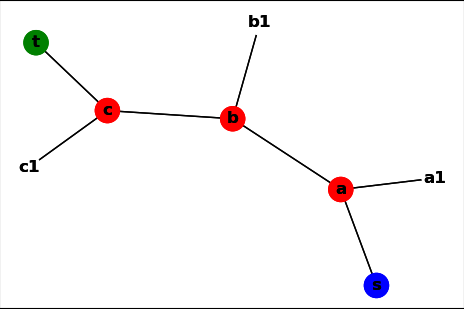
\includegraphics[scale=1]{graf.png}
		\end{center}
		\caption{Primer postavke problema planiranja kretanja u grafu}
		\label{fig:slika1}
	\end{figure}
	
	\vspace*{3\baselineskip}
	\section{Opis algoritma}
	\label{sec:prvoPoglavlje}
	\par U radu je dat predlog rešenja korišćenjem genetskog algoritma. Prvi, i jedan od najvažnijih koraka u genetskom algoritmu jeste određivanje načina na koji 
	će jedinka (hromozom) biti predstavljena. Od reprezentacije hromozoma značajno zavisi ponašanje algoritma. Nakon toga, najčešće nasumično, generiše se početna populacija koja se sastoji od određenog broja jedinki. U narednom koraku, računa se kvalitet svake jedinke, tj. funkcija prilagođenosti, a na osnovu nje se vrši selekcija najprilagođenijih jedinki iz populacije. Potom se nad selektovanim jedinkama primene genetski operatori ukrštanja i mutacije, kojima se formiraju nove generacije, sve dok se ne dostigne neki kriterijum zaustavljanja i pronađe najbolje rešenje u datom trenutku.
	
	\subsection{Reprezentacija jedinke}
	\label{subsec:podnaslov1}
	Pri generisanju početne populacije, razmatrani su različiti načini predstavljanja rešenja. U većini prethodnih radova autori predlažu hromozom u obliku koordinata pozicija robota, ili putanje od početnog do krajnjeg čvora. 
	Takva reprezentacija se nije dobro pokazala u našem slučaju, s obzirom na to da se prepreke mogu kretati na isti način kao i robot, kao i da postoji samo jedan put od čvora S do čvora T, jer je u pitanju aciklički graf.
	\par Početnu populaciju u našem algoritmu čine jedinke koje predstavljaju neku nasumičnu putanju, odnosno niz različitih validnih poteza, koji počinju od početnog stanja grafa. Preciznije, jedinka se sastoji od pokreta robota ili prepreka, koji su predstavljeni preko izvornog čvora, ciljnog čvora, težine puta između ta dva čvora i liste koja predstavlja celu putanju. Na primer, potez od čvora A do čvora B je u obliku četvorke ('A', 'B', 1, ['A', 'B']). U slučaju pomeranja prepreka, dozvoljeni su potezi težine i veće od 1, jer je prethodno dokazano da kada je potrebno da se prepreka premesti u neki slobodan čvor (koji joj nije susedan), broj poteza je isti kao i dužina puta između ta dva čvora. Ono što je bitno u tom slučaju je da je na kraju tih poteza stanje grafa takvo da je slobodan polazni čvor, a ciljni zauzet preprekom \cite{glavni}.
	\par Svaka od putanja u populaciji kreće od početnog stanja i zatim se za svaki naredni potez robota ili prepreke najpre razmatra da li je potez validan iz trenutnog stanja grafa, tj. trenutne pozicije prepreka i robota. Generiše se lista svih mogućih poteza iz trenutnog stanja i nasumično bira jedan iz liste. Zatim se izvrši taj potez i dobija se novo stanje grafa. Ako je novo stanje takvo da se robot nalazi u ciljnom čvoru, ne traže se naredni mogući potezi, jer je pronađeno rešenje. Ako je to stanje već ranije bilo razmatrano za tu jedinku, takav potez ne dodajemo u nju, jer ne želimo da se stanja ponavljaju. Može se desiti da se ovakvim nasumičnim dodavanjem istroše sva moguća stanja grafa i da više ne može da se doda nijedan potez.
	Iz tog razloga, dužina hromozoma neće biti fiksna, jer postoje slučajevi kada više neće biti validnih poteza iz nekog stanja. Maksimalna dužina jednog hromozoma ChromosomeLength određena je tako da bude proizvod dužine putanje od početnog čvora do ciljnog čvora, u oznaci P, i broja prepreka O koje se nalaze na toj putanji. \newline
	
	$ ChromosomeLength =  P * O $  \newline
	
	
	\subsection{Funkcija prilagođenosti}
	% TODO !!!!!!!!!!!!!!!!!!!!!!!!!!!!!!!!!!!!!!!!!!!!
	\label{sec:drugoPoglavlje}
	Svakoj jedinki dodeljuje se skor, čija visina ukazuje na prilagođenost jedinke. Skor se računa na osnovu poteza koji čine tu jedinku, i stanja grafa nakon tih izvršenih poteza, odnosno mesta na kojima se nalaze prepreke i robot nakon što su potezi izvršeni. Najpre se proverava da li je trenutno stanje robota jednako ciljnom čvoru T. Ukoliko se robot nalazi na cilju, skoru se dodaje neki određeni visok broj. Zatim se provera da li je robot lociran na glavnoj putanji između početnog i ciljnog čvora, za šta se takođe dodaje određena vrednost na postojeći skor. Uz to, ukoliko se na tom putu nalazi neka prepreka, za svaku od njih se skor umanjuje za određenu vrednost. Ukoliko se nijedna prepreka ne nalazi na glavnom putu, a uz to je i ciljni čvor T slobodan, skor se povećava za određenu vrednost. Povrh toga, proverava se i da li jedinka sadrži pomenute nevalidne vrednosti koje se javljaju kada su ispunjena sva moguća stanja, i od skora se oduzima određena vrednost. Na kraju, od skora se oduzima i težina cele putanje jedinke pomnožena nekim faktorom. U nastavku je dat kod funkcije koja računa taj skor.
	\vspace*{1\baselineskip}
	\lstinputlisting[language=Python, caption = Fitnes funkcija]{fitness.py}
	
	\subsection{Selekcija}	
	Pri selekciji, vrši se izbor jedinki iz trenutne populacije za reprodukciju. U našem radu korišćena je turnirska selekcija. Turnirska selekcija podrazumeva da jedinke učestvuju u turnirima, a u svakom od njih, najbolje prilagođena jedinka se proglašava pobednikom. Veličina turnira zadata je parametrom tournament\_size. U listu selektovanih jedinki se dodaju pobednici turnira sve dok veličina liste ne dostigne parametar reproduction\_size. 
	\vspace*{1\baselineskip}
	\lstinputlisting[language=Python, caption = Turnirska selekcija]{selection.py}
	
	
	\subsection{Kreiranje nove generacije}	
	\label{sec:trecePoglavlje}
	
	Pri kreiranju nove generacije, korišćena je strategija elitizma. Njome se obezbeđuje da se kvalitet rešenja ne smanjuje iz generacije u generaciju, tako što se uvek u narednu generaciju direktno prenosi određeni broj najbolje prilagođenih jedinki. U našem algoritmu, broj elitnih jedinki je velik (na primer, polovina veličine populacije) jer se pri generisanju populacije stvaraju veoma nasumične jedinke, s obzirom da se pri svakom potezu u potpunosti menja stanje grafa, odnosno menja se svaki mogući legitimni potez. Na ostale jedinke u populaciji koje ne prelaze direktno u narednu generaciju, primenjuje se operator ukrštanja, tako što se od prethodno selektovanih jedinki odabiraju dve nasumično, i one postaju roditelji. U ukrštanje će ulaziti samo jedinke koje su veće od neke minimalne dužine.
	\vspace*{1\baselineskip}
	\lstinputlisting[language=Python, caption = Generisanje nove generacije]{newgen.py}
	
	\subsubsection{Ukrštanje}
	\label{subsec:podnaslov2}
	
	Kako postoji velik broj elitnih jedinki, ukrštanje se vrši nad manjim brojem jedinki iz populacije. U našem algoritmu korišćeno je jednopoziciono ukrštanje, tako što je roditelj čija je putanja kraća presečen na nasumično odabranoj poziciji \textit{i}. Deo poteza do \textit{i} iz prvog roditelja mora da se izvrši da se dobije novo stanje grafa. Nakon toga, polazi se od \textit{i-te} pozicije u drugom roditelju i za svaki pojedinačan potez proverava da li je moguć iz prethodno dobijenog stanja. Ovde nastaje problem, jer svaki put mora da se izvrši i doda novi potez na trenutno stanje, čime se dobija potpuno novo stanje. U velikom broju slučajeva potezi iz drugog roditelja neće biti mogući u datom stanju. Tada se dete dopunjava dokle god može. Tako dete koje nastaje često bude lošijeg kvaliteta od samog roditelja. Upravo iz tog razloga i koristimo elitizam sa tako velikim procentom. Ukrštanje mnogo koplikuje situaciju, jer za svaki novi potez iz drugog roditelja mora da se proverava da li je moguć u odnosu na \textit{sve} prethodne, i samo ako jeste, može da se doda jedan potez, a već za sledeći možda opet neće biti moguće. Paremetri funkcije ukrštanja su
	prvi roditelj, drugi roditelj, stanje prepreka, stanje robota, graf, ciljni čvor, veličina populacije i putanja od prvog do poslednjeg čvora.
	\vspace*{1\baselineskip}
	\lstinputlisting[language=Python, caption = Ukrštanje]{cross.py}
	
	
	\subsubsection{Mutacija}
	\label{subsec:podnaslov3}
	Mutacija podrazumeva malu promenu genoma koja se dešava sa jako malom verovatnoćom, a koja omogućava različitost u narednoj generaciji i izbegavanje zaglavljivanja u lokalni optimum. U našem slučaju, mutacija će biti jednostavno dodavanje samo jednog poteza iz liste svih mogućih u trenutnom stanju, nakon izvršenih poteza do tog trenutka. Putanje su se nekad skraćivale u ukrštanju, pa će ih dodavanje jednog poteza možda unaprediti tako što će nastaviti kretanje, i možda u sledećem ukrštanju dozvoliti da se put produži.
	\vspace*{1\baselineskip}
	\lstinputlisting[language=Python, caption = Mutacija]{mutation.py}
	


	\subsection{Prikaz algoritma}
	\label{sec:cetvrtoPoglavlje}
	U nastavku je dat kod funkcije koja radi optimizaciju, odnosno objedinjuje sve prethodno opisane korake i izvršava ih sve dok nije postignut kriterijum zaustavljanja, koji je odabran da bude neki maksimalan broj iteracija. Ako se naiđe na dovoljno dobro rešenje, ono koje ima dovoljno visok skor iz pomenute fitnes funkcije pre nego što se generišu sve generacije, izlazi se iz petlje i vraća se to dovoljno dobro rešenje. Parametri funkcije su stanje prepreka o, stanje robota r, graf graph, ciljni čvor t, i putanja od početnog do ciljnog čvora path.
	\vspace*{1\baselineskip}
	\lstinputlisting[language=Python, caption = Genetski algoritam]{solver.py}
	
	\vspace*{3\baselineskip}
	\section{Rezultati}

	
	\vspace*{3\baselineskip}
	\section{Zaključak}
	\label{sec:zakljucak}

	\newpage
	\addcontentsline{toc}{section}{Literatura}
	\bibliography{seminarski} 
	\bibliographystyle{plain}
	
\end{document}
